\subsection{Introduction}

An increasing number of atmospheric dynamical cores are being developed to maximize efficiency on massively parallel systems, paving the way towards regionally high-resolution ($\Delta x = 50$ km or less), or even globally high resolution simulations \citep{Z2014QJRMS,HETAL2016JCLIM,DCMIP16,LetAl2018JAMES}. Incorporating these advances into Atmospheric General Circulation Models (AGCMs) requires the development of physical parameterizations appropriate for the diversity of grid configurations that dynamical cores are now able to support, referred to as scale-aware physics. The most common approach to understand and develop scale-aware physics has been through the lens of limited area, cloud resolving simulations \citep{PC2008JAS,AW2013JAS,SZ2018JCLIM}. In filtering cloud resolving solutions to some target, lower resolution resembling an AGCM grid, and studying how the filtered moments vary as a function of target grid resolution, one may develop a more general relationship between resolved and unresolved scales. While this approach is likely necessary for developing scale-aware physics, it is not sufficient. The equations of motions of motion have inherent scale dependencies \citep{O1981JAS,WETAL1997MWR,PG2006JAS,J2017JAMES}, and the resolved dynamics act accordingly to the scales a grid is able to support. Scale-aware physics should also accommodate these dependencies.

The sensitivity of the Community Atmosphere Model (CAM) to horizontal resolution is well documented over the last few decades \citep{KW1991JGR,WETAL1995CD,W1999T,W2008TELLUS,LETAL2011TELLUS,RJ2011MWR,RETAL2012ASL,OETAL2013JCLIM,RETAL2013JCLIM,ZetAl2014JCb,LETAL2015JCLIM}. The general tendency is for the atmosphere to become drier and less cloudy, the deep convection scheme less active and the magnitude of resolved vertical motion greater with increasing resolution. \cite{HR2017JCLIM,HR2018JAMES} analyzed a set of CAM simulations and found that resolved updrafts dominate the vertical velocity field of tropical convecting systems at resolutions typical of present day global models ($208.5 km \geq \Delta x \geq 27.8 km$). The scale of resolved updrafts are collocated in the horizontal with the buoyancy produced by grid-scale clouds (also referred to as stratiform clouds in the literature), and are grid limited, conforming to the effective resolution of the model ($5-10\Delta x$). Assuming that there is a characteristic buoyancy length scale associated with a grid resolution, and it is proportional to $\Delta x$, the ratio of the vertical velocity scale of that grid resolution $W$ to a high-resolution reference simulation $W_{ref}$ is:
\begin{equation}
\alpha = \frac{W}{W_{ref}} = \frac{\Delta x_{ref}}{\Delta x} , \label{eq:eq6-1}
\end{equation}
where $\Delta x_{ref}$ is the grid-spacing of a high-resolution reference, and it is assumed that the magnitude and height scale of the buoyancy is unchanged or compensating across resolutions. The physical interpretation of equation~\ref{eq:eq6-1} is a rising column of buoyancy creates a low pressure perturbation of similar horizontal scale in its wake, and this pressure gradient scales like $\Delta x^{-1}$, facilitating convergence into the pressure minimum and the resultant vertical velocity also scales like $\Delta x^{-1}$. While \cite{HR2017JCLIM} found that equation~\ref{eq:eq6-1} over-predicted the change in vertical velocity across resolutions in their aqua-planet simulations, \cite{HR2017JCLIM} discovered that this over-prediction was at least in-part, due to time-truncation errors arising from too small a physics time-step, $\Delta t_{phys}$, in the higher resolution simulations.

In this study, it is shown that through scaling $\Delta t_{phys}$ in a manner which avoids large time-truncation errors at higher resolutions {Herrington et al., in review), the analytical scaling in equation~\ref{eq:eq6-1} does explain the change in vertical velocities across resolutions in an aqua-planet configuration using CAM. The implications of equation~\ref{eq:eq6-1} are that for a doubling of the resolution, CAM can simulate the same resolved mass flux in half the area. Grid-scale cloud fraction and regions of ascent are then confined to a smaller areas at higher resolutions; the area and magnitude of subsiding motion also increases with resolution. Greater subsiding motion results in a drier and more stable atmosphere, which reduces the frequency the deep convection scheme is triggered. Section $6.2$ describes the model and experimental design, section 6.3 presents results and section 6.3 provides the conclusions.

\subsection{Methods}

\subsection{Results}

The probability density function (PDF) of negative, or upward vertical pressure velocities $\omega$ in the aqua-planets are shown in Figure~\ref{fig:2pdf}a. The magnitude of upward $\omega$ increases in a monotonic way with resolution, with positive, or downward $\omega$ behaving similarly (not shown). The PDF's may be scaled to the high-resolution $ne120$ resolution, through $P(\omega)_s = \alpha P (\omega / \alpha)$, where $\alpha$ is the scale factor equation~\ref{eq:eq6-1}. The scaled PDF's all line up on top of the high-resolution reference (Figure~\ref{fig:2pdf}b); equation~\ref{eq:eq6-1} explains the variation in vertical velocity across resolutions to first order. 

\begin{figure}[t]
\begin{center}
\noindent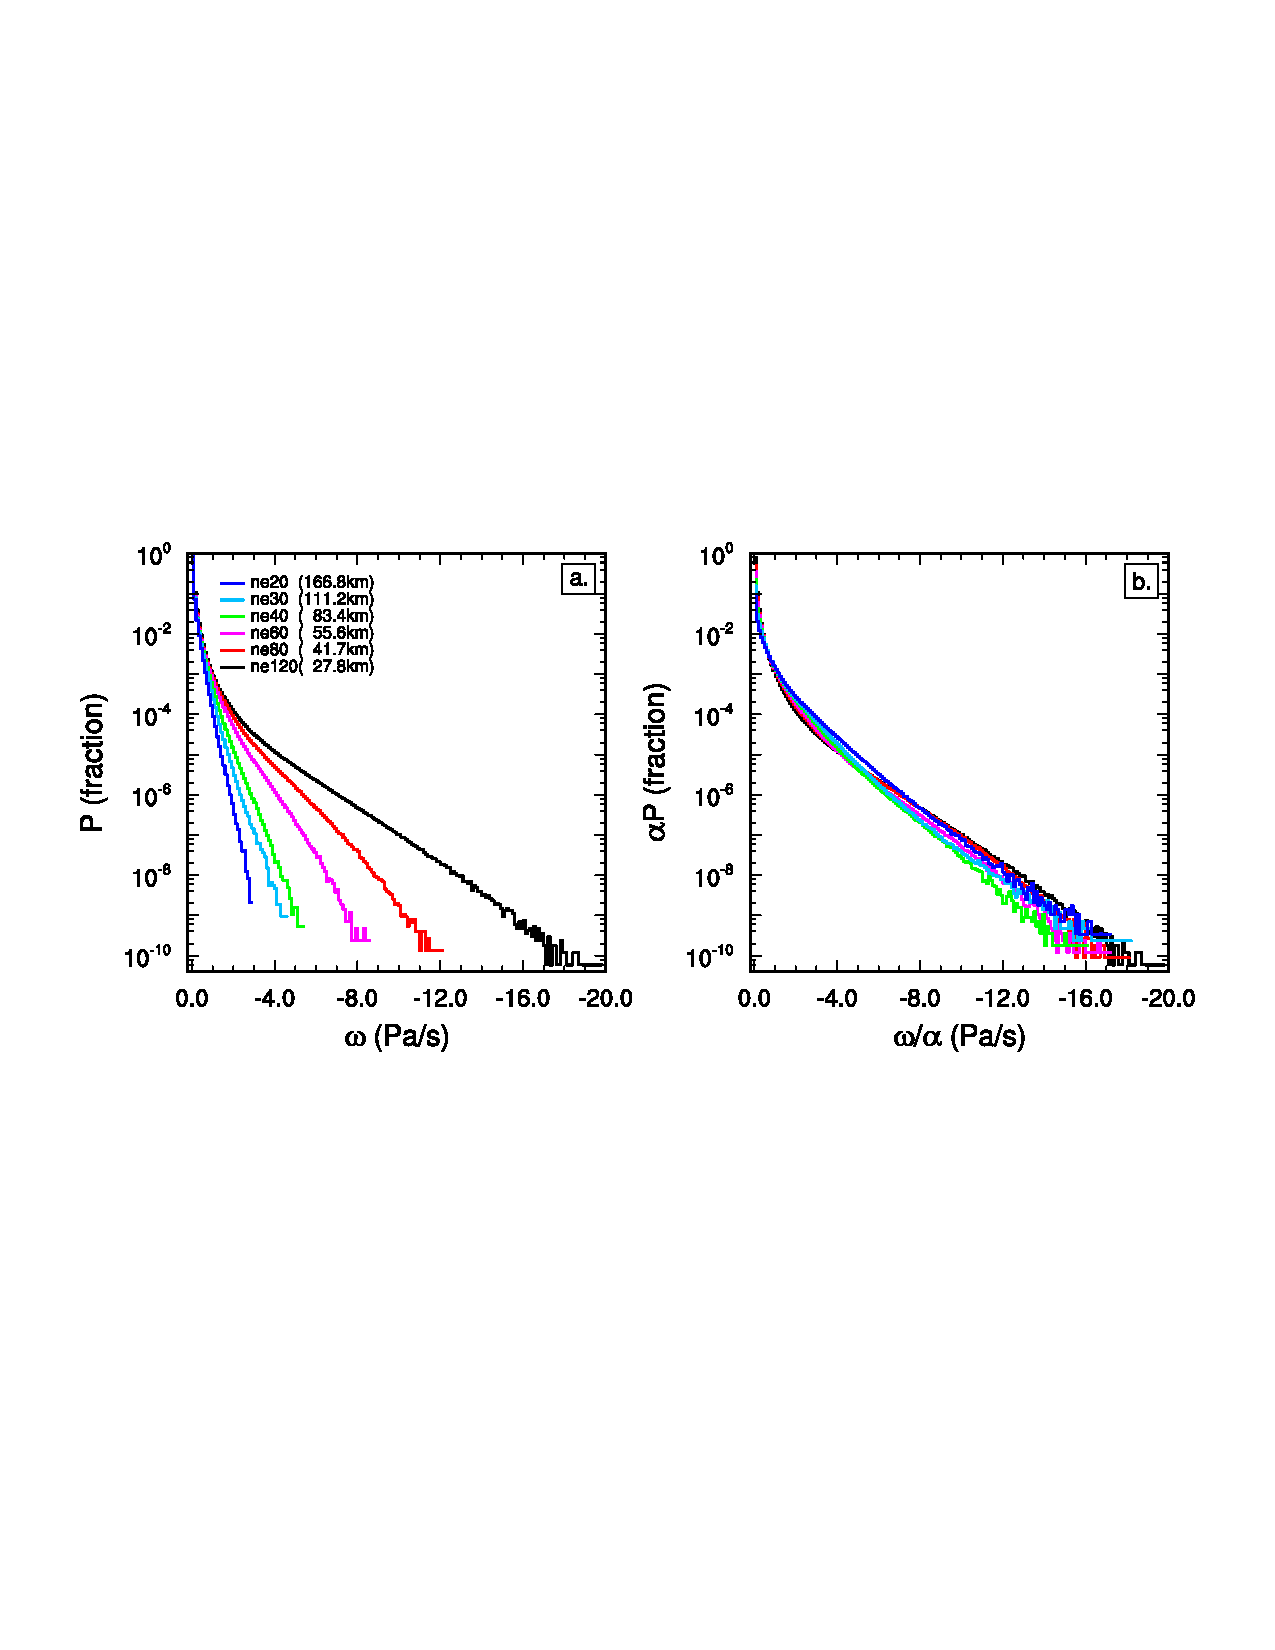
\includegraphics[width=35pc,angle=0]{chapter6/temp_2pdf.pdf}\\
\end{center}
\caption{}
\label{fig:2pdf}
\end{figure}

The impact of the changing vertical velocity field on the global mean state can be understood through decomposing the mass weighted global mean $\omega$ into upward and downward components,
\begin{equation}
\overline{\langle \omega \rangle} = \overline{\langle f_{u} \rangle} \, \overline{\langle \omega_{u} \rangle} + \overline{\langle f_{d} \rangle} \, \overline{\langle \omega_{d} \rangle}, \label{eq:eq6-2}
\end{equation}
where $\langle f_x \rangle$ and $\langle \omega_x \rangle$ refers to the mass weighted fraction and mass weighted mean $\omega$, respectively, subscript $u$ refers to upward motion and $d$, downward motion; the overbars indicate is a time mean global mean. This components of equation~\ref{eq:eq6-2} are shown in Figure~\ref{fig:8panel}a,b,e,f for the six aqua-planet simulations. The magnitude of both $\overline{\langle \omega_{u} \rangle}$ and $\overline{\langle \omega_{d} \rangle}$ increase monotonically with resolution, the upward component increasing more than the downward component. In contrast, $\overline{\langle f_{u} \rangle}$ decreases with resolution while $\overline{\langle f_{d} \rangle}$ increases, although in both cases there is a reversal in this trend in the highest resolution simulation, $ne120$. Note that the magnitude of the change in $\overline{\langle f_{u} \rangle}$ and $\overline{\langle f_{d} \rangle}$ is small, a range of about $0.015$ across all simulations. Figure~\ref{fig:8panel}e,g shows that the products  $\overline{\langle f_{u} \rangle} \, \overline{\langle \omega_{u} \rangle}$ and $\overline{\langle f_{d} \rangle} \, \overline{\langle \omega_{d} \rangle}$ are equal and opposite, which is a requirement of mass conservation in the model and a convenient check of the calculation. Besides the six aqua-planets described in Section 6.2, 23 additional year-long aqua-planet experiments were carried out at various resolutions, with modified parameters in the dynamical core and the physics. The spread in the components of equation~\ref{eq:eq6-2} in the simulations with perturbed parameters is relatively large for $\overline{\langle f_{x} \rangle}$, compared with $\overline{\langle \omega_{x} \rangle}$.

\begin{figure}[t]
\begin{center}
\noindent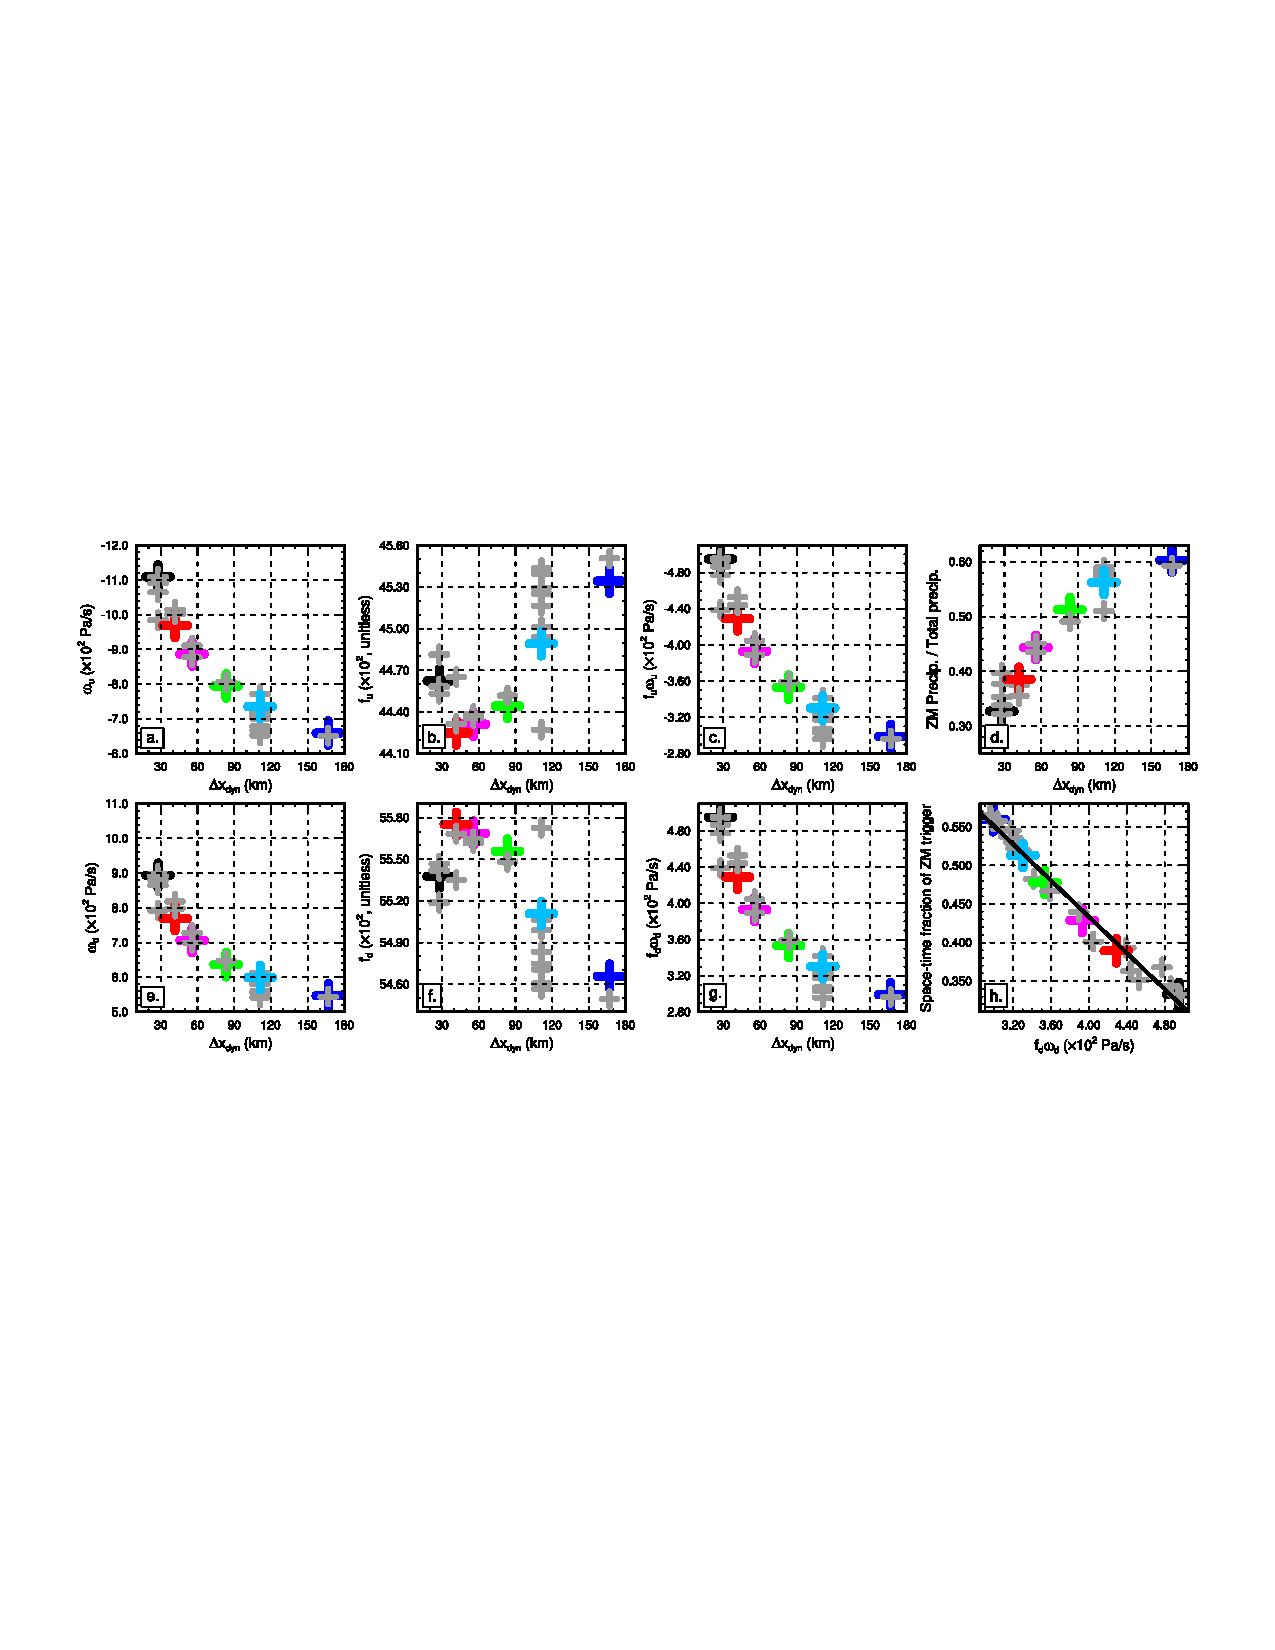
\includegraphics[width=40pc,angle=0]{chapter6/temp_diags_8panel.pdf}\\
\end{center}
\caption{}
\label{fig:8panel}
\end{figure}

It is common for the activity of deep convection scheme to become less active with increasing resolution in CAM. This is depicted in Figure~\ref{fig:8panel}d, which shows the global mean fraction of total precipitation arising from the deep convective scheme ({\em{ZM scheme}}) decreasing from about $0.60$ at low resolution ($ne20$) to about $0.32$ at high resolution ($ne120$). The global mean space time fraction the ZM scheme is triggered (hereafter referred to as FREQZM) is highly negatively correlated with $\overline{\langle f_{d} \rangle} \, \overline{\langle \omega_{d} \rangle}$ in the 29 simulations (Pearson's R-value = 0.99; Figure~\ref{fig:8panel}h), more then with any individual component of equation~\ref{eq:eq6-2}. 

\begin{figure}[t]
\begin{center}
\noindent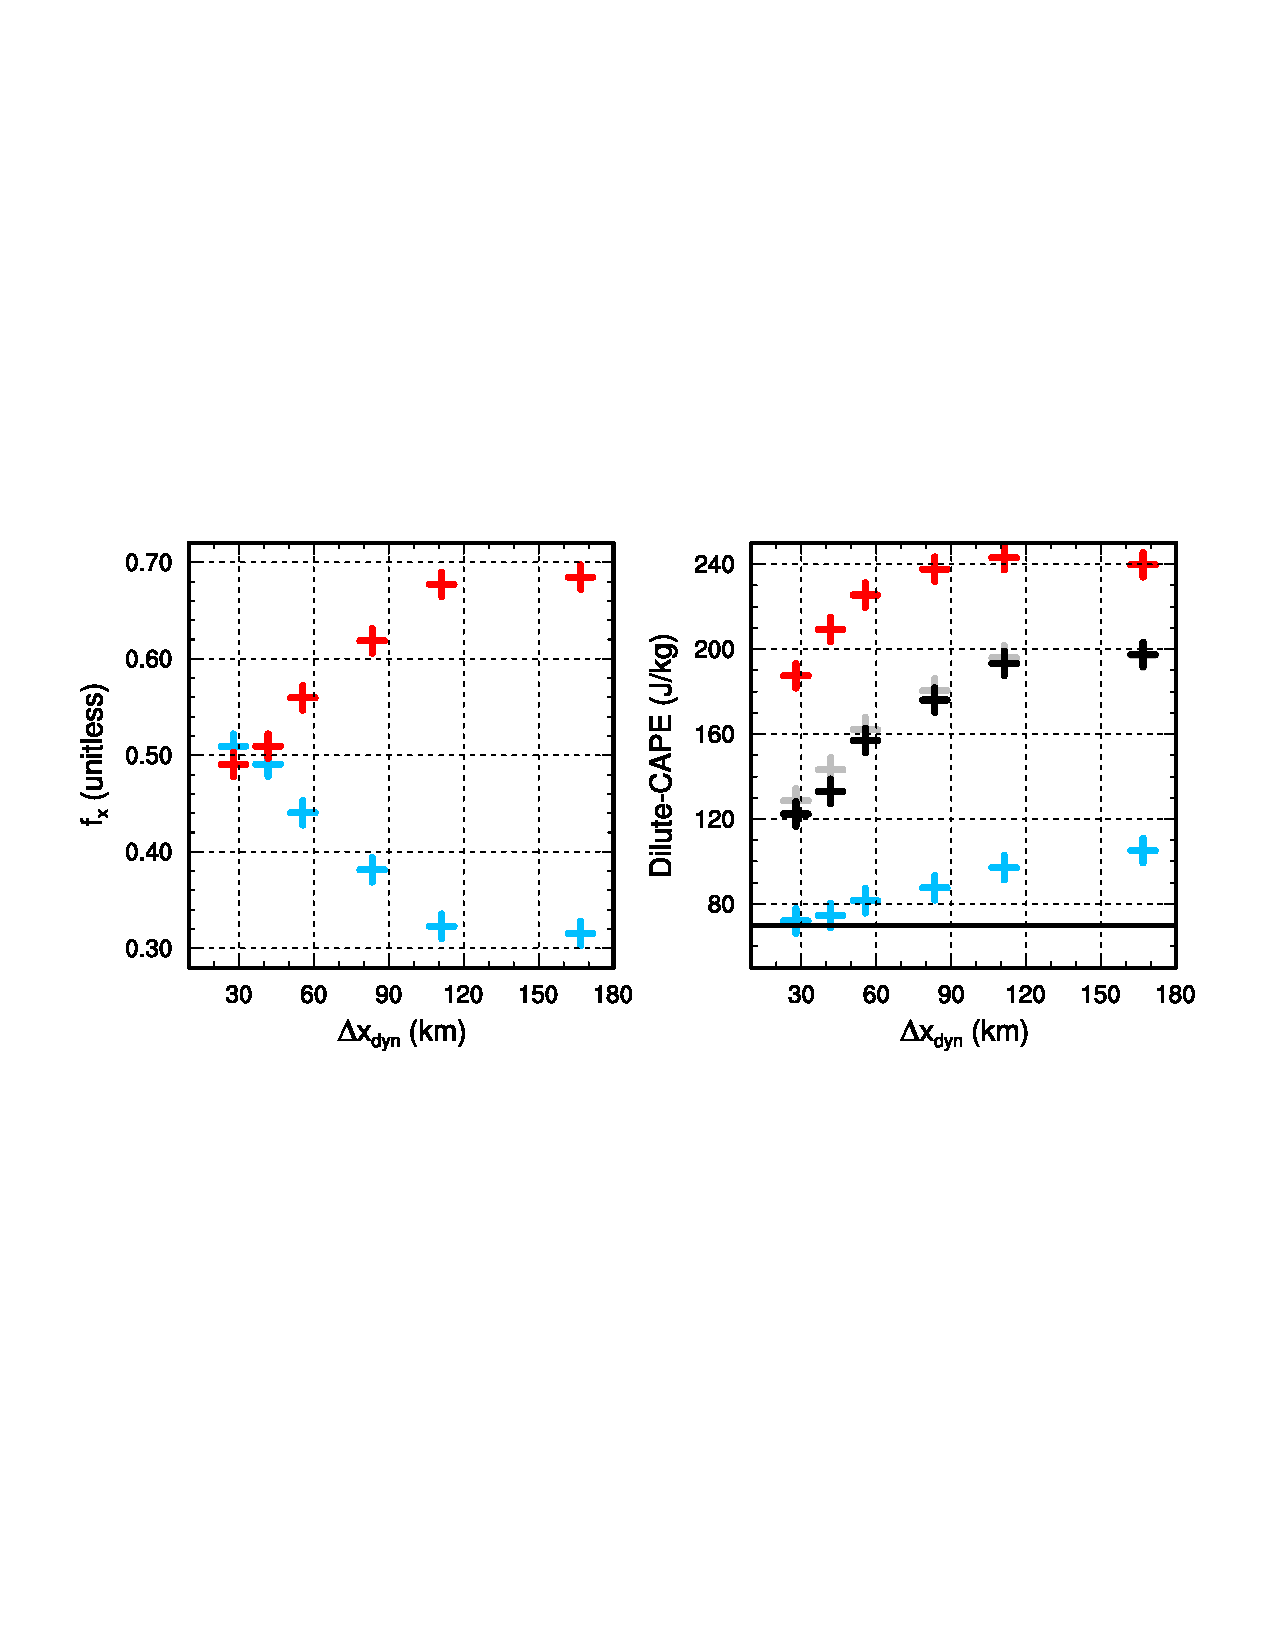
\includegraphics[width=20pc,angle=0]{chapter6/temp_cape.pdf}\\
\end{center}
\caption{}
\label{fig:vomg}
\end{figure}

Figure~\ref{fig:vomg} shows how these highly correlated quantities, the time mean $\langle f_{d} \rangle \langle \omega_{d} \rangle$ and FREQZM, look in the zonal mean. The ZM scheme is most active in the deep tropics, equatorward of about $10^{\circ}$, decreasing sharply poleward throughout the subtropics and mid-latitudes, and increasing again at high latitudes ($\geq 60^{\circ}$). $\langle f_{d} \rangle \langle \omega_{d} \rangle$ is smallest in the deep tropics (equatorward of about $10^{\circ}$), increasing sharply poleward, throughout the subtropics and then decreasing in the middle latitudes ($40^{\circ}$) and throughout polar regions. FREQZM largely mirrors that pattern, with more frequent activity where $\langle f_{d} \rangle \langle \omega_{d} \rangle$ is small. The correspondence between these two quantities with resolution do not appear to have a zonal structure; $\langle f_{d} \rangle \langle \omega_{d} \rangle$  increases and FREQZM decreases everywhere in proportion with one another across resolutions.

The ZM trigger uses a dilute form of CAPE, and is consistent with the negative relation between $\overline{\langle f_{d} \rangle} \, \overline{\langle \omega_{d} \rangle}$ and FREQZM in the zonal mean, and across resolutions. In the classical, non-dilute case, CAPE can be broken into two main components \citep{Z2002JGR}; instability due to the thermodynamic state of parcels in the boundary layer and the instability generated through advection of dry static energy and moisture by the environment, i.e., the resolved flow. The latter term generally contributes positively to CAPE in regions of ascent and negatively in regions of subsidence, which is consistent with Figure~\ref{fig:vomg}.

\begin{figure}[t]
\begin{center}
\noindent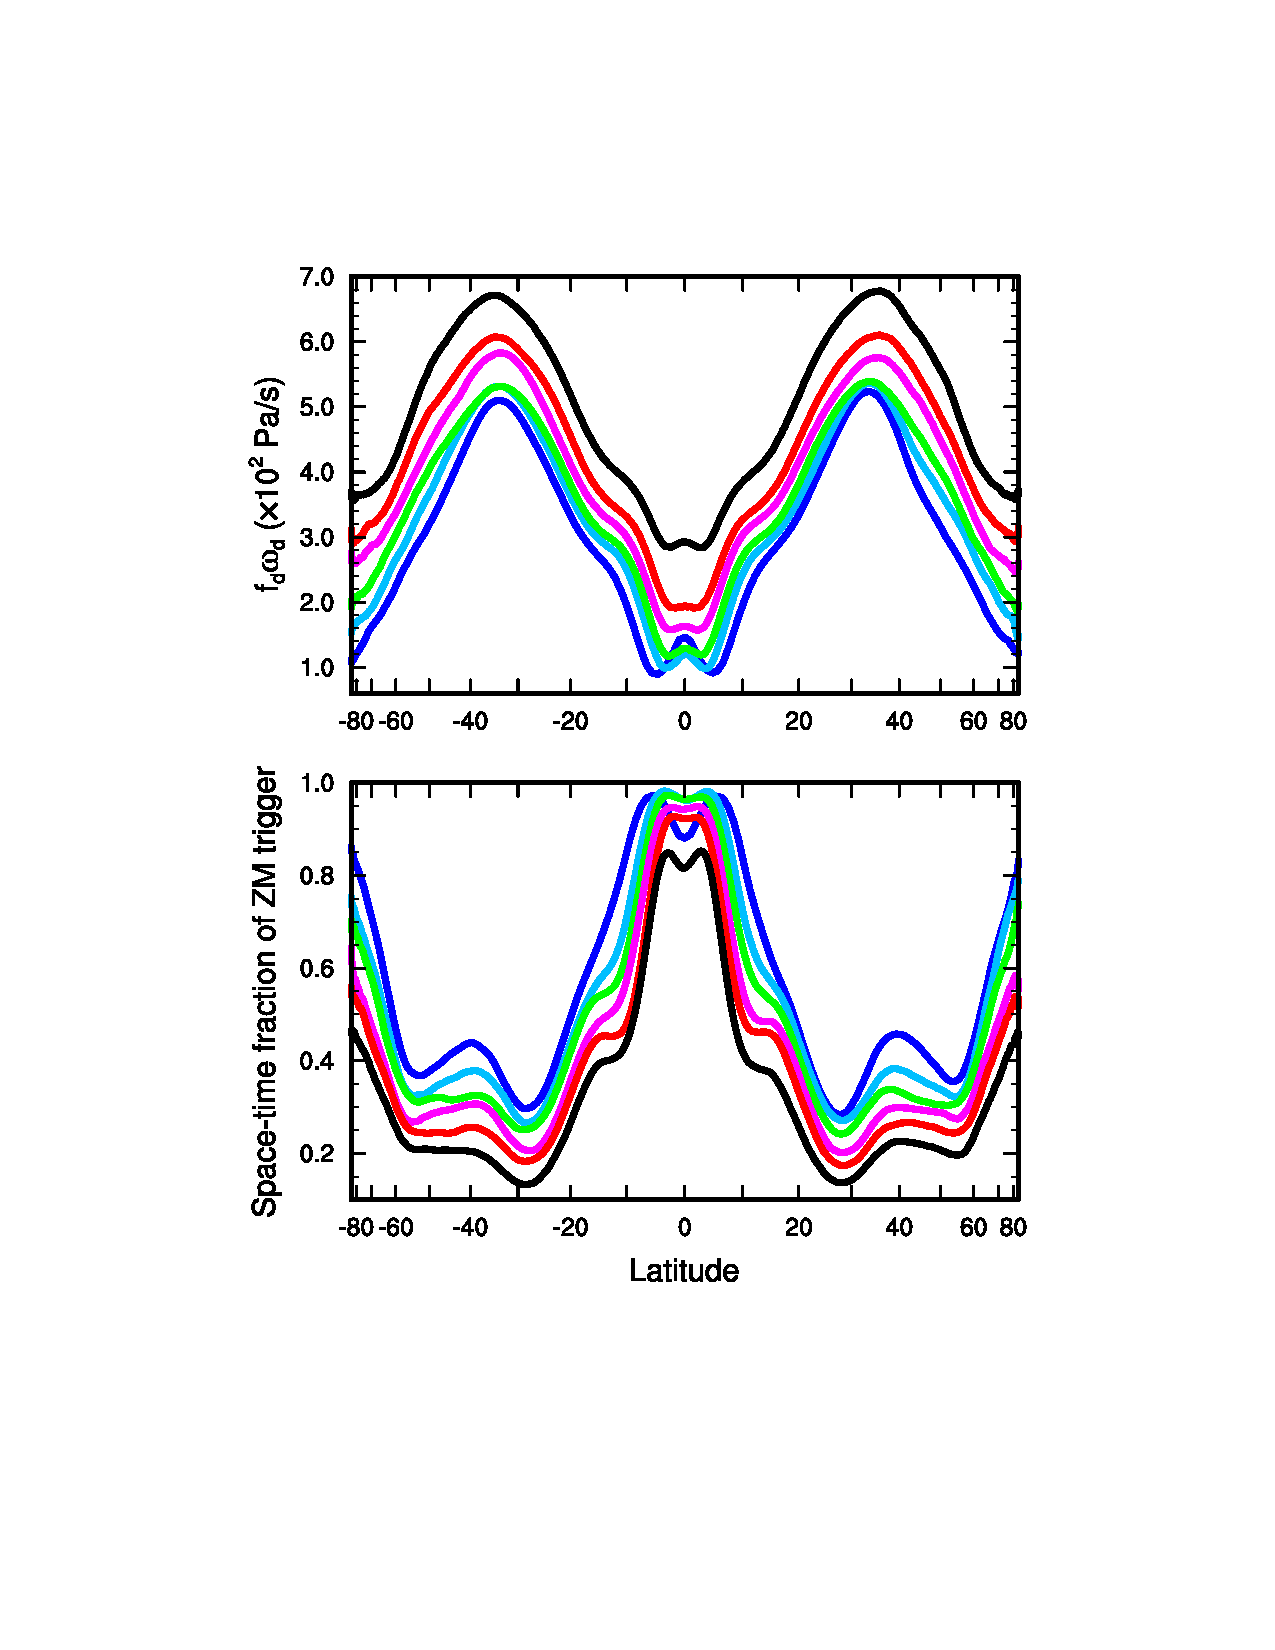
\includegraphics[width=20pc,angle=0]{chapter6/temp_zonal_fracd*vomgd.pdf}\\
\end{center}
\caption{}
\label{fig:vomg}
\end{figure}

To further support the supposed negative relation between subsiding motion and CAPE, temperature and moisture profiles are collected from the deep tropics of the simulations, and conditionally sampled depending on whether $\langle \omega \rangle$ is positive or negative, indicating predominantly subsiding or ascending grid columns. The mean temperature and moisture profiles of subsiding and ascending regions are then used to compute the dilute-CAPE used by the ZM scheme, offline. Figure~\ref{fig:cape}b indicates that regions ascent are associated with high value of CAPE in the mean ($>170$ J/kg), and low values in subsiding regions ($>110$ J/kg), due to an anomolous warming layer in the $600-800$ hPa layer, and anomalous moisture deficit throughout the entire column, relative to the mean (not shown). Figure~\ref{fig:cape}a shows that fractional area of air columns in the deep tropics that are subsiding (ascending) changes drastically with resolution, from $0.3$ ($0.7$) in the $ne20$ run, and monotonically increasing (decreasing) with resolution to $0.7$ ($0.3$) in the $ne120$ run. Interestingly, the sum of the product of the fractional areas with their corresponding CAPE values (grey crosses in Figure~\ref{fig:cape}b) gives approximately the same value as the CAPE value resulting from the mean temperature and moisture profiles over the entire deep tropics. The CAPE values in the deep tropics are decreasing with resolution because a larger fraction subsiding columns make up a larger portion of the region with resolution.

\begin{figure}[t]
\begin{center}
\noindent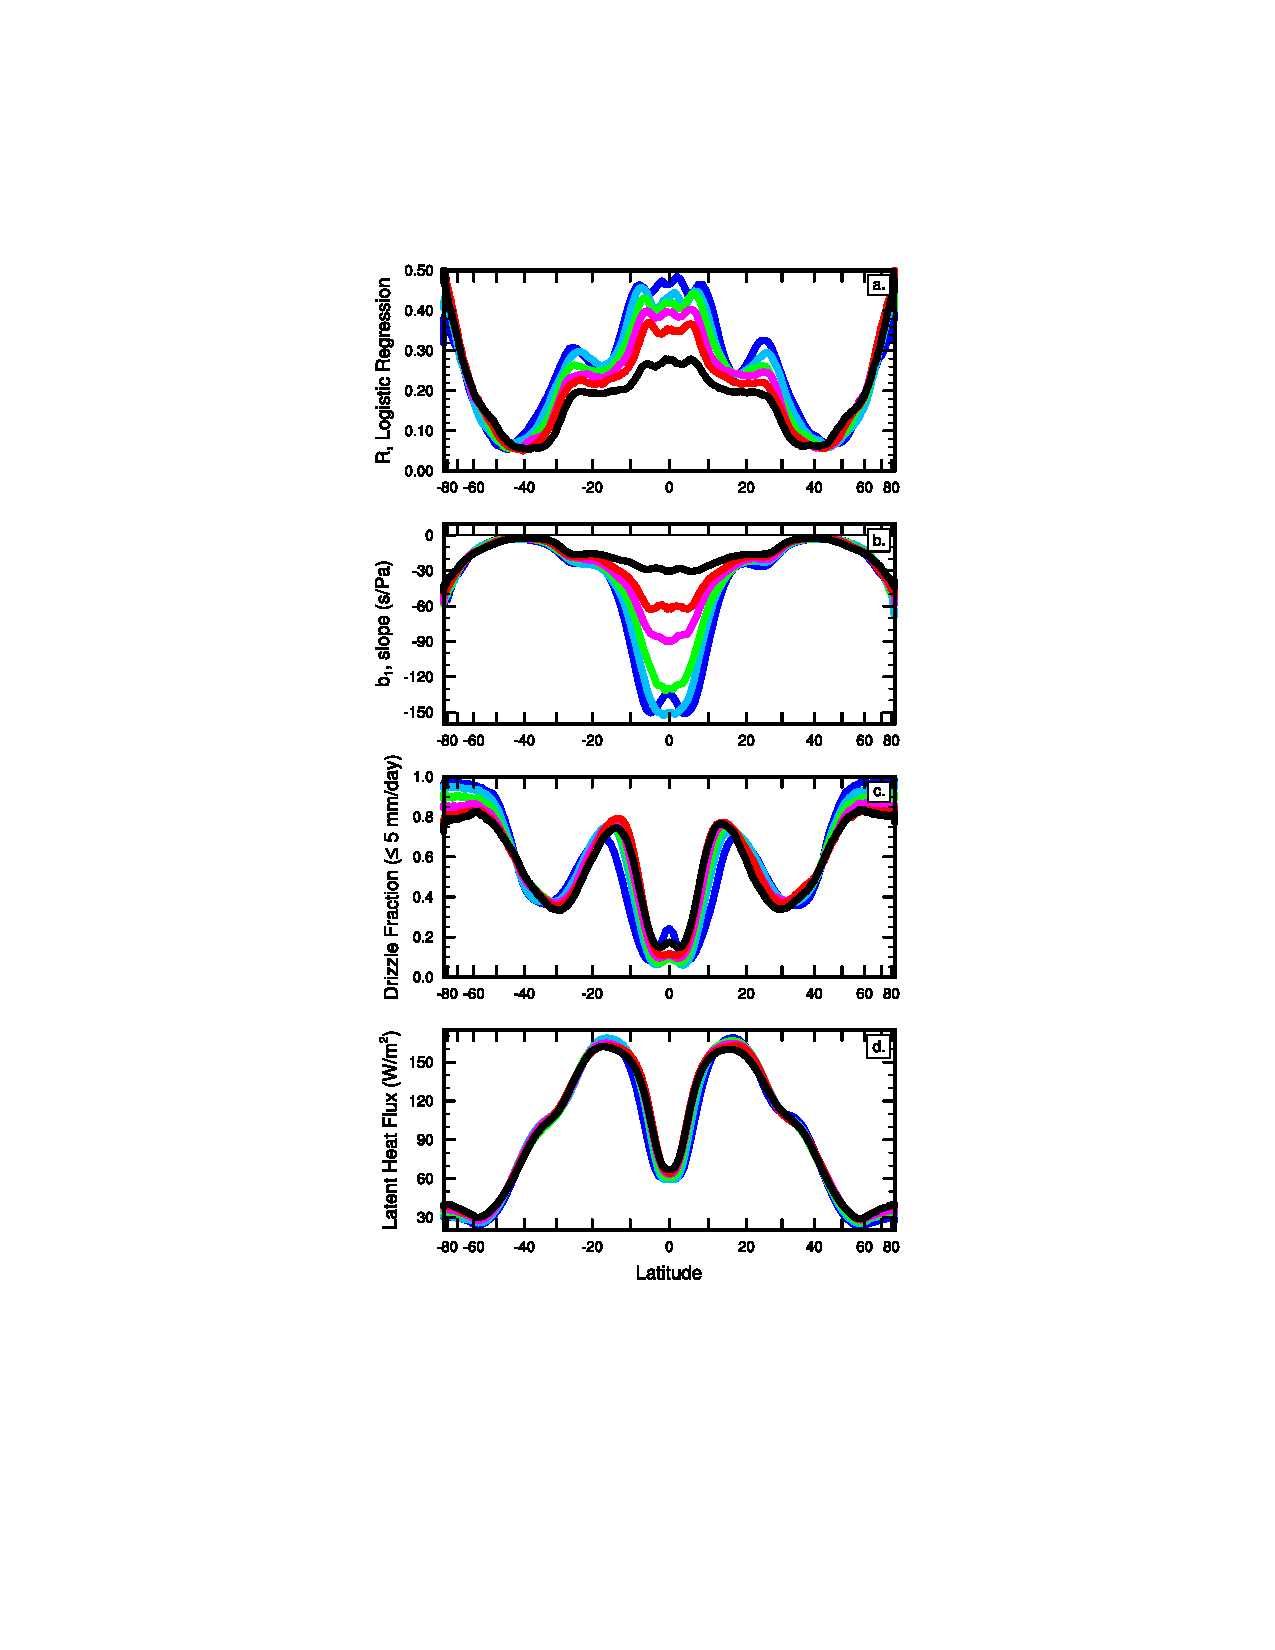
\includegraphics[width=14pc,angle=0]{chapter6/temp_zonal_4reg_dwn.pdf}\\
\end{center}
\caption{}
\label{fig:4reg}
\end{figure}

To further understand how the relationship manifests within the simulations themselves, a logistic regression is performed for each grid column in the simulations. Logistic regression uses an iterative method to fit a continuous variable predictor, $x$ to a binary predictand $p$ \citep{},
\begin{equation}
p = \frac{exp{[b_0 + b_1 x]}}{1 + exp{[b_0 + b_1 x]}}, \label{eq:eq6-3}
\end{equation}
where $b_0$ and $b_1$ are the shape parameters of the exponential. The predictor is chosen as the instantaneous $\langle f_{d} \rangle \langle \omega_{d} \rangle$ of a grid column, and the predictand is whether or not the ZM scheme is active, $1$ for yes and $0$ for no. Since the aqua-planets have zonally symmetric boundary conditions, there is a zonally varying structure in the goodness of fit (R-value) and parameter $b_1$ (hereafter referred to as the sensitivity parameter). Figure~\ref{fig:4reg}a,b, shows the zonal mean R-values and sensitivity parameter, which indicates the goodness of fit is greatest in the deep tropics. Figure~\ref{fig:4reg}d shows the time mean zonal mean latent heat flux in the simulations, which is expected to increase CAPE through the component associated with the thermodynamic state of boundary layer parcels. In the deep tropics, the latent heat flux is small, and the sensitivity parameter is large and negative, indicating that subsiding motion is successfully depressing CAPE, and the activity of the ZM scheme.

Poleward of $10^{\circ}$, the R-value decreases to a local minimum between $10^{\circ} - 15^{\circ}$ latitude, and the magnitude of the sensitivity parameter steeply declines. Even though the subsiding motion is increasing polewards of $10^{circ}$, this motion is less effective in depressing the convection scheme. The local minimum in the R-value corresponds with a local maximum in the latent heat fluxes, indicating that the ZM scheme is primarily responding to the instability of the boundary layer due to large surface latent heat fluxes. The CAPE values in this region ($10^{\circ} - 15^{\circ}$) latitude are likely to be small, since ZM precipitation rate consists of mostly drizzle (Figure~\ref{fig:4reg}c). It is likely the preponderance of drizzle in this region is a result of the largely subsiding motion (Figure~\ref{fig:vomg}) constraining CAPE form becoming too large. AGCMs are known to suffer from an excess drizzle bias \citep{} in this approximate region, and this analysis indicates that the drizzle bias is in CAM is due to the use of a CAPE closure in the ZM scheme.   

\subsection{Conclusions}